% =====================================================================
\chapter{Tester la stationnarité et le retour à la moyenne}
\label{ch:3}
% =====================================================================

\section{Objectifs et organisation du chapitre}

\paragraph{Objectifs.} Les chapitres précédents ont utilisé le test ADF comme une boîte noire. Ce chapitre l'ouvre. À la fin, vous saurez : (1) écrire la régression de Dickey-Fuller et expliquer pourquoi sa statistique ne suit pas une loi de Student ; (2) choisir les termes déterministes (constante, tendance) et le nombre de retards ; (3) évaluer la puissance d'un test et la relier au nombre de demi-vies observées ; (4) utiliser le test KPSS et combiner les deux ; (5) calculer et interpréter le ratio de variance et l'exposant de Hurst ; (6) appliquer ces outils à deux paires réelles et lire correctement des résultats contradictoires.

\paragraph{Code.} \texttt{code/ch03/ch03\_stationarity\_tests.py}, expériences E1 à E6.

% =====================================================================
\section{Le test de Dickey-Fuller}
% =====================================================================

\subsection{La régression}

On part de l'AR(1) $x_t = c + \varphi x_{t-1} + \varepsilon_t$ et l'on soustrait $x_{t-1}$ des deux côtés :
\[
\Delta x_t = c + \gamma\,x_{t-1} + \varepsilon_t, \qquad \gamma = \varphi - 1.
\]
L'hypothèse nulle $H_0 : \gamma = 0$ (soit $\varphi = 1$) est celle d'une \emph{racine unitaire} : le processus est une marche aléatoire, sans retour à la moyenne. L'alternative $H_1 : \gamma < 0$ est celle d'un processus stationnaire. La statistique de test est le rapport $\tau = \hat\gamma/\widehat{\mathrm{se}}(\hat\gamma)$, calculé exactement comme un $t$ de Student.

\begin{intuition}
On demande aux données : \og quand $x$ était haut hier, a-t-il eu tendance à baisser aujourd'hui ?\fg. Si oui ($\hat\gamma$ nettement négatif), il y a une force de rappel. La subtilité est de savoir ce que veut dire \og nettement\fg{} quand, sous l'hypothèse nulle, la série elle-même erre sans borne.
\end{intuition}

\subsection{Pourquoi la statistique n'est pas normale}

Plaçons-nous sous $H_0$ dans le cas le plus simple (pas de constante, $x_0 = 0$) : $x_t = x_{t-1}+\varepsilon_t$. L'estimateur est $\hat\gamma = \sum x_{t-1}\varepsilon_t/\sum x_{t-1}^2$. Regardons le numérateur. En élevant au carré $x_t = x_{t-1}+\varepsilon_t$ :
\[
x_t^2 = x_{t-1}^2 + 2x_{t-1}\varepsilon_t + \varepsilon_t^2 \quad\Longrightarrow\quad x_{t-1}\varepsilon_t = \tfrac12\big(x_t^2 - x_{t-1}^2 - \varepsilon_t^2\big).
\]
En sommant de $t = 1$ à $n$, la somme des $x_t^2 - x_{t-1}^2$ \og télescope\fg{} (chaque terme s'annule avec le suivant) et il reste
\[
\sum_{t=1}^n x_{t-1}\varepsilon_t = \tfrac12\Big(x_n^2 - \sum_{t=1}^n\varepsilon_t^2\Big).
\]
Divisons par $n\sigma^2$. Par la proposition~\ref{c1:prop:rw}, $x_n/(\sigma\sqrt n)$ suit une loi $\N(0,1)$ (exactement, si les chocs sont gaussiens) ; notons-la $W$. Par la loi des grands nombres, $\frac1{n\sigma^2}\sum\varepsilon_t^2 \to 1$. Donc
\[
\frac{1}{n\sigma^2}\sum_{t=1}^n x_{t-1}\varepsilon_t \;\longrightarrow\; \tfrac12\,(W^2 - 1).
\]
Or $W^2$ suit une loi du $\chi^2$ à un degré de liberté, très asymétrique : $\Prob(W^2 < 1) = \Prob(|W|<1) \approx 68\,\%$. Le numérateur de $\hat\gamma$ est donc négatif dans environ deux cas sur trois \emph{alors même qu'il n'y a aucun retour à la moyenne}. La statistique $\tau$ est décalée vers la gauche par rapport à une loi normale. La théorie complète \citep{dickeyfuller1979,hamilton1994} montre que $\tau$ converge vers une fonctionnelle du mouvement brownien, $\tfrac12(W(1)^2-1)/\sqrt{\int_0^1 W(r)^2\,\dd r}$, dont les quantiles se calculent par simulation.

\begin{codebox}[ — E1, distribution de Dickey-Fuller]
\textbf{Protocole :} 20\,000 marches aléatoires de 500 points ; statistique $\tau$ avec constante. \textbf{Résultats :} quantiles à 1\,\%, 5\,\% et 10\,\% : $-3{,}44$ ; $-2{,}87$ ; $-2{,}57$, pour des valeurs tabulées de $-3{,}43$ ; $-2{,}86$ ; $-2{,}57$. La moyenne de $\tau$ vaut $-1{,}54$ au lieu de 0. Si l'on utilisait par erreur le seuil de la loi normale ($-1{,}645$), on conclurait à tort au retour à la moyenne dans $46{,}4\,\%$ des cas.
\end{codebox}

\begin{figure}[h]
\centering
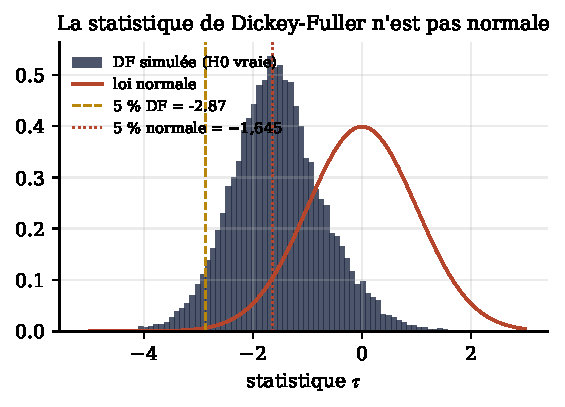
\includegraphics[width=0.6\textwidth]{ch03/dickey_fuller_distribution.pdf}
\caption{Distribution simulée de la statistique de Dickey-Fuller sous l'hypothèse de racine unitaire, comparée à la loi normale.}
\label{c3:fig:df}
\end{figure}

\subsection{Termes déterministes et valeurs critiques}

Les valeurs critiques dépendent de ce que l'on met dans la régression :

\begin{table}[h]
\centering\small
\caption{Valeurs critiques asymptotiques du test de Dickey-Fuller (statistique $\tau$).}
\label{c3:tab:crit}
\begin{tabular}{lccc}
\toprule
Régression & 1\,\% & 5\,\% & 10\,\% \\
\midrule
Sans constante : $\Delta x_t = \gamma x_{t-1} + \varepsilon_t$ & $-2{,}58$ & $-1{,}95$ & $-1{,}62$ \\
Avec constante : $\Delta x_t = c + \gamma x_{t-1} + \varepsilon_t$ & $-3{,}43$ & $-2{,}86$ & $-2{,}57$ \\
Avec constante et tendance : $\Delta x_t = c + \delta t + \gamma x_{t-1} + \varepsilon_t$ & $-3{,}96$ & $-3{,}41$ & $-3{,}13$ \\
\bottomrule
\end{tabular}
\end{table}

\paragraph{Lequel choisir ?} Pour un \emph{spread} de \emph{pairs trading} dont la moyenne n'est pas nulle, on met une constante. On ajoute une tendance seulement si une raison économique la justifie, comme un écart de frais de gestion entre deux ETF (section~\ref{c3:sec:cases}) ; ajouter une tendance \og au cas où\fg{} réduit la puissance.

\subsection{Le test augmenté (ADF)}

Si les chocs du \emph{spread} sont eux-mêmes autocorrélés, $\varepsilon_t$ n'est pas un bruit blanc et le test est faussé. Le test de Dickey-Fuller augmenté ajoute des retards de la variation :
\[
\Delta x_t = c + \gamma x_{t-1} + \sum_{j=1}^{p}\delta_j\,\Delta x_{t-j} + \varepsilon_t.
\]
Les retards absorbent l'autocorrélation de court terme ; les valeurs critiques asymptotiques restent celles du tableau~\ref{c3:tab:crit}. On choisit $p$ par un critère d'information (AIC ou BIC), ce que fait \texttt{statsmodels} avec \texttt{autolag="AIC"}.

% =====================================================================
\section{La puissance : combien de données faut-il ?}
% =====================================================================

La \emph{puissance} d'un test est la probabilité de rejeter $H_0$ quand elle est fausse. Ici : la probabilité de détecter un retour à la moyenne qui existe vraiment.

\begin{codebox}[ — E2, puissance du test ADF à 5\,\%]
\textbf{Protocole :} AR(1) stationnaires, 200 à 400 répétitions par case. \textbf{Résultats :} tableau~\ref{c3:tab:power} et figure~\ref{c3:fig:power}.
\end{codebox}

\begin{table}[h]
\centering\small
\caption{Probabilité que le test ADF (constante, 1 retard) rejette la racine unitaire à 5\,\%.}
\label{c3:tab:power}
\begin{tabular}{lccccc}
\toprule
 & $n = 100$ & $250$ & $500$ & $1\,000$ & $2\,500$ \\
\midrule
$\varphi = 0{,}90$ (demi-vie 6,6) & 29\,\% & 96\,\% & 100\,\% & 100\,\% & 100\,\% \\
$\varphi = 0{,}95$ (demi-vie 13,5) & 11\,\% & 44\,\% & 96\,\% & 100\,\% & 100\,\% \\
$\varphi = 0{,}98$ (demi-vie 34,3) & 9\,\% & 13\,\% & 33\,\% & 85\,\% & 100\,\% \\
$\varphi = 0{,}99$ (demi-vie 69,0) & 7\,\% & 6\,\% & 10\,\% & 32\,\% & 97\,\% \\
\bottomrule
\end{tabular}
\end{table}

\begin{figure}[h]
\centering
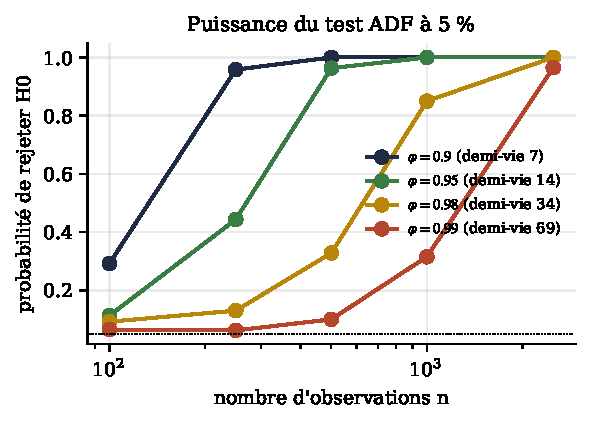
\includegraphics[width=0.6\textwidth]{ch03/puissance_adf.pdf}
\caption{Puissance du test ADF en fonction de la taille d'échantillon, pour quatre vitesses de retour.}
\label{c3:fig:power}
\end{figure}

\paragraph{La règle des demi-vies.} Les cases de puissance comparable ont un point commun : la quantité $n(1-\varphi)$. Avec $n(1-\varphi) = 10$ ($\varphi = 0{,}90$, $n = 100$ ; ou $\varphi = 0{,}99$, $n = 1\,000$), la puissance est d'environ 30\,\% ; avec $n(1-\varphi) = 25$ ($\varphi = 0{,}95$, $n=500$ ; ou $\varphi = 0{,}99$, $n = 2\,500$), elle dépasse 95\,\%. Or, d'après la proposition~\ref{c1:prop:hl}, $n(1-\varphi) \approx \ln 2 \times n/h_{1/2}$ : ce qui compte n'est pas le nombre de points, mais le \emph{nombre de demi-vies observées}. Règle pratique : il faut observer au moins une trentaine de demi-vies pour détecter un retour à la moyenne de façon fiable.

\begin{pitfall}
Passer de données quotidiennes à des données minute multiplie le nombre de points mais pas le nombre de demi-vies : si l'écart revient en 30 jours, une année de données minute contient toujours une douzaine de demi-vies, et le test reste peu puissant. Augmenter la fréquence n'aide que si la dynamique de retour est elle-même rapide.
\end{pitfall}

% =====================================================================
\section{Le test KPSS : inverser l'hypothèse nulle}
% =====================================================================

Le test ADF a pour hypothèse nulle la non-stationnarité ; ne pas la rejeter ne prouve pas qu'elle est vraie (manque de puissance). \citet{kpss1992} proposent l'inverse : $H_0$ = stationnarité. Le modèle est $x_t = \xi t + r_t + u_t$, où $r_t$ est une marche aléatoire de variance d'innovation $\sigma_r^2$ et $u_t$ est stationnaire ; $H_0 : \sigma_r^2 = 0$.

La statistique repose sur les sommes partielles des résidus $e_t$ de la régression de $x_t$ sur une constante (ou une constante et une tendance) : $S_t = \sum_{i\le t} e_i$, et
\[
\eta = \frac{1}{n^2}\,\frac{\sum_{t=1}^n S_t^2}{\hat\sigma^2_{LR}},
\]
où $\hat\sigma^2_{LR}$ est une variance de long terme estimée à la Newey-West (chapitre~2). Valeur critique à 5\,\% : $0{,}463$ (constante), $0{,}146$ (constante et tendance).

\begin{intuition}
Les écarts d'une série stationnaire s'annulent en moyenne : leur somme cumulée oscille autour de zéro, comme les dépenses et recettes d'un ménage bien géré. Ceux d'une série non stationnaire s'accumulent : la somme cumulée part au loin, comme une dette qui grossit. KPSS mesure la taille de cette somme cumulée.
\end{intuition}

\begin{codebox}[ — E3, combiner ADF et KPSS]
\textbf{Protocole :} 400 séries de 500 points par processus ; tests à 5\,\%. \textbf{Résultats :} marche aléatoire : ADF n'est pas rejeté et KPSS est rejeté dans 89\,\% des cas (conclusion correcte \og non stationnaire\fg). AR(1) avec $\varphi = 0{,}5$ : ADF rejeté, KPSS non rejeté dans 94\,\% des cas (conclusion correcte \og stationnaire\fg). AR(1) avec $\varphi = 0{,}95$ : les deux tests rejettent dans 40\,\% des cas, signe que la série est stationnaire mais très persistante.
\end{codebox}

\begin{table}[h]
\centering\small
\caption{Lecture conjointe des tests ADF et KPSS.}
\label{c3:tab:decision}
\begin{tabular}{lll}
\toprule
 & KPSS non rejeté & KPSS rejeté \\
\midrule
ADF rejeté & stationnaire (signal clair) & persistante, à confirmer \\
ADF non rejeté & données insuffisantes & non stationnaire (signal clair) \\
\bottomrule
\end{tabular}
\end{table}

% =====================================================================
\section{Le ratio de variance}
% =====================================================================

\subsection{Définition et calcul pour l'AR(1)}

Le ratio de variance compare la variance des variations sur $q$ périodes à $q$ fois la variance des variations sur une période :
\[
VR(q) = \frac{\Var(x_{t+q} - x_t)}{q\,\Var(x_{t+1}-x_t)}.
\]
Pour une marche aléatoire, $\Var(x_{t+q}-x_t) = q\sigma^2$ (proposition~\ref{c1:prop:rw}), donc $VR(q) = 1$.

\begin{proposition}\label{c3:prop:vr}
Pour un AR(1) stationnaire, $VR(q) = \dfrac{1-\varphi^q}{q\,(1-\varphi)}$, qui est strictement inférieur à 1 pour $0<\varphi<1$ et $q\ge2$.
\end{proposition}
\begin{proof}
Par la proposition~\ref{c1:prop:varspread} avec $\beta = 1$ et la proposition~\ref{c1:prop:ar1} : $\Var(x_{t+q}-x_t) = \gamma(0) + \gamma(0) - 2\gamma(q) = 2\gamma(0)(1-\varphi^q)$. De même, $\Var(x_{t+1}-x_t) = 2\gamma(0)(1-\varphi)$. Le rapport donne la formule. Comme $1-\varphi^q = (1-\varphi)(1+\varphi+\dots+\varphi^{q-1})$ et que chaque $\varphi^j < 1$ pour $j \ge 1$, on a $1-\varphi^q < q(1-\varphi)$.
\end{proof}

\begin{intuition}
Pour une marche aléatoire, les mouvements s'additionnent : dix jours bougent $\sqrt{10}$ fois plus qu'un jour. Pour un processus qui revient à la moyenne, les mouvements se compensent : dix jours bougent moins que ce que l'addition prédirait, $VR < 1$. Pour un processus qui suit une tendance, ils se renforcent : $VR > 1$.
\end{intuition}

\citet{lomackinlay1988} en déduisent un test : sous l'hypothèse de marche aléatoire à chocs homoscédastiques,
\[
z(q) = \frac{VR(q) - 1}{\sqrt{2(2q-1)(q-1)/(3qn)}}
\]
suit approximativement une loi $\N(0,1)$.

\begin{codebox}[ — E4, ratio de variance]
\textbf{Protocole :} séries de 5\,000 points. \textbf{Résultats :} pour l'AR(1) avec $\varphi = 0{,}9$, $VR(q)$ simulé vaut $0{,}954$ ; $0{,}823$ ; $0{,}655$ ; $0{,}417$ ; $0{,}224$ ; $0{,}150$ pour $q = 2, 5, 10, 20, 40, 60$, contre $0{,}950$ ; $0{,}819$ ; $0{,}651$ ; $0{,}439$ ; $0{,}246$ ; $0{,}166$ en théorie. Pour une série dont les rendements sont autocorrélés positivement (coefficient 0,3), $VR(10) = 1{,}77$. Statistique $z(10)$ : $-1{,}25$ (marche aléatoire, non significatif), $-7{,}21$ (AR), $+16{,}0$ (rendements autocorrélés). Pour la marche aléatoire, $VR(60) = 0{,}73$ : l'erreur-type de $VR(60)$ vaut environ $0{,}125$ ici, c'est un écart de deux erreurs-types dû au hasard, rappel que les grands horizons sont mal mesurés.
\end{codebox}

\begin{figure}[h]
\centering
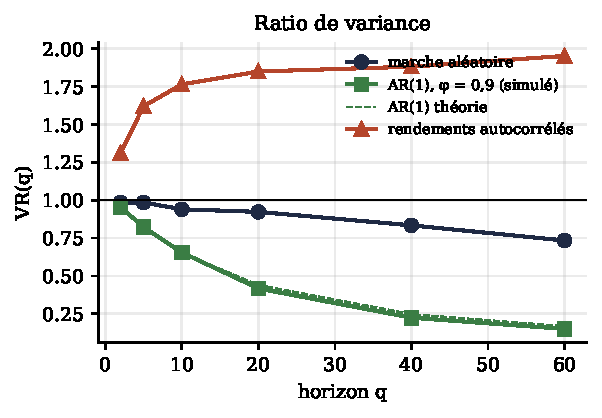
\includegraphics[width=0.6\textwidth]{ch03/ratio_variance.pdf}
\caption{Ratio de variance en fonction de l'horizon pour trois dynamiques.}
\label{c3:fig:vr}
\end{figure}

% =====================================================================
\section{L'exposant de Hurst}
% =====================================================================

L'exposant de Hurst $H$ résume la façon dont l'amplitude des variations croît avec l'horizon : $\mathrm{sd}(x_{t+\tau} - x_t) \propto \tau^H$. On l'estime par la pente de la régression de $\log\mathrm{sd}(x_{t+\tau}-x_t)$ sur $\log\tau$. Pour une marche aléatoire, $H = 1/2$ ; $H < 1/2$ indique un retour à la moyenne ; $H > 1/2$ une persistance des tendances \citep{chan2013}.

\begin{codebox}[ — E5, exposant de Hurst (retards 2 à 50)]
\textbf{Protocole :} 200 séries de 2\,000 points. \textbf{Résultats} (moyenne, et intervalle 5–95\,\%) : marche aléatoire $0{,}494$ $[0{,}44\,;\,0{,}55]$ ; AR(1) $\varphi=0{,}9$ : $0{,}218$ $[0{,}19\,;\,0{,}26]$ ; AR(1) $\varphi=0{,}99$ : $0{,}457$ $[0{,}40\,;\,0{,}51]$ ; rendements autocorrélés : $0{,}525$ $[0{,}47\,;\,0{,}58]$.
\end{codebox}

\begin{pitfall}
L'exposant de Hurst n'est pas une propriété intrinsèque : il dépend de la plage de retards choisie. Sur les retards 2 à 50, un AR(1) de demi-vie 69 jours ($\varphi = 0{,}99$) a un $H$ indiscernable de celui d'une marche aléatoire : le retour à la moyenne ne se manifeste qu'au-delà de la demi-vie. C'est le même problème de puissance que pour ADF, sous un autre nom. Utilisez Hurst et le ratio de variance comme diagnostics descriptifs, jamais comme tests uniques.
\end{pitfall}

% =====================================================================
\section{Études de cas réelles}\label{c3:sec:cases}
% =====================================================================

On applique les outils à deux écarts construits sur 500 séances réelles (octobre 2024 à octobre 2026).

\begin{table}[h]
\centering\small
\caption{Diagnostics de stationnarité sur données réelles (E6). ADF avec AIC ; KPSS avec retards automatiques ; $p$-valeurs KPSS bornées entre 0,01 et 0,10 par la table.}
\label{c3:tab:cases}
\begin{tabular}{lcccccc}
\toprule
Série & ADF $p$ & KPSS $p$ & $\hat\varphi$ & demi-vie (j) & $VR(10)$ & $H$ \\
\midrule
$\log$ GLD (un prix seul) & 0,547 & 0,01 & 0,9949 & 136,6 & 0,79 & 0,46 \\
$\log$ GLD $-$ $\log$ GLDM, constante seule & 0,925 & 0,01 & 0,9338 & 10,1 & 0,10 & 0,01 \\
idem, tests avec tendance & $<$0,001 & $\ge$0,10 & — & — & — & — \\
idem, tendance retirée & $<$0,001 & $\ge$0,10 & 0,0111 & 0,2 & 0,10 & 0,01 \\
$\log$ KO $-$ $\log$ PEP & 0,949 & 0,01 & 0,9996 & 1\,803 & 0,96 & 0,50 \\
$\log$ KO $-$ ($-0{,}432$) $\log$ PEP (MCO) & 0,684 & 0,01 & 0,9915 & 81,4 & 0,82 & 0,44 \\
\bottomrule
\end{tabular}
\end{table}

\begin{figure}[h]
\centering
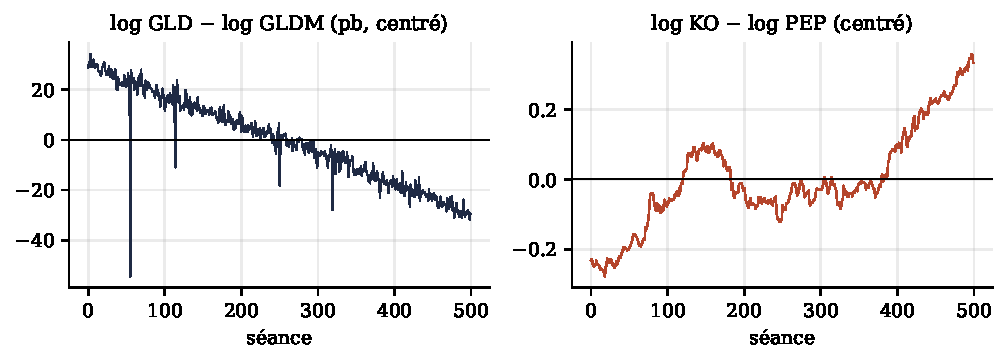
\includegraphics[width=0.95\textwidth]{ch03/cas_reels_ecarts.pdf}
\caption{À gauche, l'écart logarithmique entre GLD et GLDM en points de base : une pente régulière vers le bas plus un bruit quotidien de quelques points de base. À droite, l'écart logarithmique entre KO et PEP : une dérive sans retour.}
\label{c3:fig:cases}
\end{figure}

\paragraph{GLD et GLDM : un quasi-arbitrage parfaitement arbitré.} Les deux fonds détiennent de l'or physique. Avec une constante seule, ADF ne rejette pas la racine unitaire ($p = 0{,}925$) et KPSS rejette la stationnarité : conclusion naïve, \og non stationnaire\fg. C'est faux. Le log-ratio décroît régulièrement de $0{,}293\,\%$ par an : c'est l'ordre de grandeur de l'écart entre les frais de gestion annuels des deux fonds, prélevés jour après jour sur l'actif du fonds le plus cher. Avec une tendance dans la régression, ADF rejette massivement ($\tau = -22$) et KPSS ne rejette plus. Une fois la tendance retirée, l'écart a un écart-type de $4{,}5$ points de base, son quantile à 99\,\% vaut $8{,}3$ points de base, et $\hat\varphi = 0{,}011$ : un écart d'un jour a disparu le lendemain. Les participants autorisés, qui créent et détruisent des parts contre de l'or, maintiennent la relation. \textbf{Leçon :} il n'y a rien à gagner à l'échelle quotidienne après coûts ; s'il existe un avantage, il est intrajournalier et réservé à ceux qui exécutent vite et pour presque rien.

\paragraph{KO et PEP : la paire des manuels ne l'était pas.} Avec un ratio de 1 ou avec le ratio MCO (négatif, ce qui n'a aucun sens économique pour deux concurrents), l'écart ne montre aucun retour à la moyenne détectable. Le $\hat\varphi$ de $0{,}9915$ correspondrait à une demi-vie de 81 jours, soit à peine six demi-vies dans l'échantillon : le tableau~\ref{c3:tab:power} dit que, même si ce retour existait, on ne pourrait pas le détecter avec deux ans de données. Ajoutons que tester les résidus d'une régression estimée exige d'autres valeurs critiques (chapitre~4) : les $p$-valeurs de la dernière ligne sont même trop optimistes.

\section{Tests multiples : un avertissement}

Supposons que l'on teste 500 écarts candidats au seuil de 5\,\%. Même si aucun ne revient à la moyenne, on en déclarera en moyenne 25 \og stationnaires\fg. Les vrais retours à la moyenne, s'il y en a, sont noyés parmi les faux positifs, et ce sont souvent les faux positifs qui ont les meilleures statistiques en échantillon. Le chapitre~7 traite cette question (contrôle du taux de fausses découvertes) et le chapitre~16 en tire les conséquences pour l'évaluation des stratégies.

% =====================================================================
\section{Ce que la théorie apporte, et ses limites}
% =====================================================================

\paragraph{Apports.} Des valeurs critiques correctes, qui évitent de voir du retour à la moyenne partout ; un lien quantitatif entre durée d'observation et capacité de détection ; des diagnostics complémentaires (KPSS, ratio de variance, Hurst) qui, ensemble, donnent une image plus fiable qu'un test isolé.

\paragraph{Limites.} (1) Tous ces tests supposent des paramètres constants sur l'échantillon ; une rupture (changement de moyenne) fait ressembler une série stationnaire à une marche aléatoire. (2) Les tendances déterministes doivent être justifiées économiquement, sinon on teste ce qu'on veut voir. (3) Un test répond à une question statistique (\og y a-t-il une force de rappel ?\fg) ; la question économique (\og cette force est-elle assez rapide et ample pour payer les coûts ?\fg) demande une analyse séparée, comme le montre l'écart GLD/GLDM, parfaitement stationnaire et pourtant inexploitable.

% =====================================================================
\section{Fiche à recopier au tableau blanc}
% =====================================================================

\begin{whiteboard}
\begin{itemize}[leftmargin=1.2em]
\item \textbf{DF :} $\Delta x_t = c + \gamma x_{t-1} + \varepsilon_t$, $H_0 : \gamma = 0$ (racine unitaire), $\tau = \hat\gamma/\mathrm{se}$.
\item \textbf{Pourquoi non normale :} $\sum x_{t-1}\varepsilon_t = \frac12(x_n^2 - \sum\varepsilon_t^2)$ $\Rightarrow$ $\frac12(W^2-1)$, négatif 68\,\% du temps.
\item \textbf{Seuils 5\,\% :} $-1{,}95$ (rien), $-2{,}86$ (constante), $-3{,}41$ (tendance).
\item \textbf{ADF :} ajouter $\sum\delta_j\Delta x_{t-j}$, choisir $p$ par AIC.
\item \textbf{Puissance :} gouvernée par $n(1-\varphi)\approx 0{,}69\,n/h_{1/2}$ ; viser $\ge 30$ demi-vies.
\item \textbf{KPSS :} $H_0$ stationnarité ; $\eta = n^{-2}\sum S_t^2/\hat\sigma^2_{LR}$ ; seuil $0{,}463$.
\item \textbf{Ratio de variance :} $VR(q) = \Var(x_{t+q}-x_t)/(q\Var(\Delta x))$ ; AR(1) : $(1-\varphi^q)/(q(1-\varphi))$.
\item \textbf{Hurst :} $\mathrm{sd}(x_{t+\tau}-x_t)\propto\tau^H$ ; $H<\frac12$ retour, $=\frac12$ marche, $>\frac12$ tendance.
\end{itemize}
\end{whiteboard}

% =====================================================================
\section{Exercices}
% =====================================================================

\begin{exercise}
Refaites la démonstration de $\sum x_{t-1}\varepsilon_t = \frac12(x_n^2 - x_0^2 - \sum\varepsilon_t^2)$ avec $x_0 \ne 0$. Calculez $\Prob(W^2 < 1)$ à l'aide de la table de la loi normale.
\end{exercise}

\begin{exercise}
Un écart a une demi-vie estimée de 20 jours. Combien d'années de données quotidiennes faut-il pour avoir une puissance d'environ 95\,\% d'après la règle des demi-vies ? Et une demi-vie de 5 jours ?
\end{exercise}

\begin{exercise}
Calculez la limite de $VR(q)$ quand $q\to\infty$ pour un AR(1) stationnaire. Interprétez.
\end{exercise}

\begin{exercise}[à coder]
Simulez un AR(1) avec $\varphi = 0{,}8$ dont la moyenne saute de 0 à 5 au milieu de l'échantillon. Appliquez ADF et KPSS. Que concluez-vous à tort ? Comment détecter la rupture (voir chapitre~17) ?
\end{exercise}

\begin{exercise}[à coder]
Sur l'écart GLD/GLDM sans tendance, calculez l'autocorrélation des variations quotidiennes. Pourquoi est-elle proche de $-0{,}5$ quand l'écart est un bruit blanc ? (Indice : $\Var(\Delta x)$ et $\Cov(\Delta x_t,\Delta x_{t-1})$ pour un bruit blanc.)
\end{exercise}

% =====================================================================
\section{Pour aller plus loin}
% =====================================================================

\begin{toread}
\begin{itemize}[leftmargin=1.2em]
\item \citet{hamilton1994}, chapitre~17 (\og Univariate Processes with Unit Roots\fg) : la théorie asymptotique complète de Dickey-Fuller, avec les tables de valeurs critiques.
\item \citet{dickeyfuller1979} et \citet{kpss1992} : les articles originaux.
\item \citet{lomackinlay1988} : le test du ratio de variance, appliqué aux indices boursiers américains.
\item \citet{chan2013}, chapitre~2 : ADF, Hurst et ratio de variance appliqués à des paires réelles, avec code.
\end{itemize}
\end{toread}

\section{Scripts du chapitre}
\noindent\texttt{code/ch03/ch03\_stationarity\_tests.py} : E1 (figure~\ref{c3:fig:df}), E2 (tableau~\ref{c3:tab:power}, figure~\ref{c3:fig:power}), E3 (tableau~\ref{c3:tab:decision}), E4 (figure~\ref{c3:fig:vr}), E5 (Hurst), E6 (tableau~\ref{c3:tab:cases}, figure~\ref{c3:fig:cases}).
